\chapter{Antecedentes}

\section{Modelo Est\'andar}

El Modelo Est\'andar es el formalismo te\'orico-experimental que hasta el d\'{\i}a de hoy  describe con mayor precisi\'on las interacciones entre las part\'{\i}culas elementales y los diferentes tipos de fuerzas que experimentan entre las mismas. Los mayores desarrollos te\'oricos y descubrimientos experimentales que dieron forma al Modelo Est\'andar se tuvieron en la segunda mitad del siglo XX con el desarrollo de la Teor\'{\i}a Cu\'antica de Campo, fruto del esfuerzo de cient\'{\i}ficos de todo el mundo los cuales a partir de los modelos te\'oricos y observaciones experimentales construyeron una clasificaci\'on de las part\'{\i}culas en base a sus propiedades fundamentales como lo son la masa, la carga el\'ectrica, el esp\'{\i}n, entre otras. Dicha clasificaci\'on se muestra en la Figura~\ref{fig:ME}. Las part\'{\i}culas elementales est\'an divididas en dos categor\'{\i}as, los fermiones y los bosones, los fermiones est\'an a su vez divididos en quarks y leptones los cuales tienen un valor fraccional de esp\'{\i}n (1/2), adem\'as de que obedecen la estadistica de Fermi-Dirac y el principio de exclusion de Pauli. Los quarks son particulas elementales que constituyen a los hadrones, ya que debido al principio de confinamiento los quarks no pueden co-existir en estado libre.

Cuatro son las fuerzas fundamentales en la naturaleza, la fuerza electromagn\'etica, la d\'ebil, la fuerte y la gravitacional, el modelo est\'andar incluye las tres primeras, la gravitacional no esta incluida sin embargo su contribuci\'on en la f\'{\i}sica de part\'{\i}culas es despreciable si se compara por ejemplo con la fuerza electromagn\'etica (una raz\'on de $10^{36}$ en la escala de los Giga-electr\'on volts). El modelo est\'andar esta respaldado por una serie de observaciones experimentales, la mas reciente fue la observaci\'on de una nueva part\'{\i}cula cuyas propiedades son consistentes con el boson de Higgs~\cite{higgs}. Sin embargo aun existen fen\'omenos en la naturaleza que no pueden ser explicados dentro del formalismo del modelo est\'andar, ejemplo de ello es la naturaleza y composici\'on de la materia oscura.

\begin{figure}
\begin{center}
  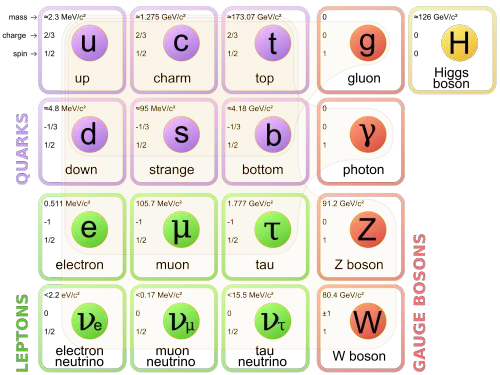
\includegraphics[width=4.0in]{standard-model.png}
  \caption{Clasificaci\'on de las particulas seg\'un el Modelo est\'andar de las part\'iculas elementales}
  \label{fig:ME}
\end{center}
\end{figure}


\section{Materia Oscura}

La materia oscura o dark matter (por su nombre en ingles) recibe este nombre debido a que no emite radiaci\'on electromagn\'etica, por lo que su existencia se infiere debido a su influencia gravitacional sobre la materia visible (o tambi\'en conocida como barionica) que se encuentra a su alrededor, dicho fen\'omeno ha sido observado en c\'umulos de galaxias en donde la velocidad de rotaci\'on de las mismas no corresponde a la que seria producida debido a la fuerza de gravedad ejercida por la materia visible a su alrededor. A pesar de los esfuerzos por parte de la comunidad cient\'{\i}fica hasta este momento se desconoce la composici\'on de la materia oscura, lo que se sabe, por medio de observaciones astron\'omicas, es que aproximadamente la materia oscura representa el 30.1\%  de la composici\'on materia-energ\'{\i}a del universo, el resto es energ\'{\i}a oscura (69.4\%) y materia visible (0.5\%). Recientemente y con el af\'an de entender la composici\'on de la materia oscura y su localizaci\'on en el universo la comunidad cient\'{\i}fica ha desarrollado varios experimentos, uno de los mas significativos es el Alpha Magnetic Spectrometer (AMS-02) el cual es un detector de particulas que tiene como uno de sus objetivos primordial el de buscar indicios de materia oscura, dicho detector fue dise\~nado y construido en el CERN para su futura instalacion en la estacion espacial internacional (ISS por sus siglas en ingles). Entre sus observaciones mas recientes~\cite{ams:cern} se ha reportado un flujo de positrones anomalo el cual una posible explicacion es el proceso de aniquilacion de particulas de materia oscura, donde en dicho proceso se libera energia en forma de positrones .  Dicho flujo anomalo puede observarse a partir de los 25~GeV en la Figura~\ref{fig:AMS_positron} donde tambien se presenta una comparacion con otros experimentos que observan similar comportamiento.

\begin{figure}
\begin{center}
 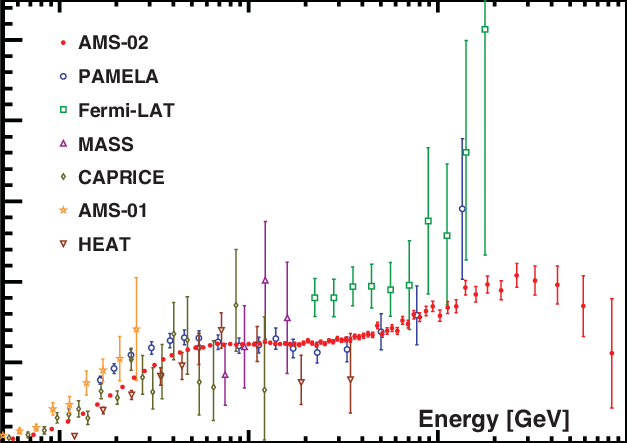
\includegraphics[width=4.0in]{AMS_positronflux.png}
  \caption{Flujo de positrones medido por el experimento AMS-02, comparado con los experimentos PAMELA,Fermi-LAT, MASS, CAPIRCE, AMS-01 y HEAT.}
 \label{fig:AMS_positron}
 \end{center}
\end{figure}

Dichas observaciones cosmologicas han motivado a los fisicos teoricos de altas energias a postular nuevos modelos en los cuales la composicion de la materia oscura se pueda entender por medio de nuevas particulas elementales, las cuales no se encuentren descritas en el modelos estandar y que podrian estar siendo producidas en los aceleradores de particulas modernos como lo es el Gran Colisionador de Hadrones en Ginebra, Suiza.  Dichos modelos propuestos entran en la categoria de extensiones al modelo estandar y por lo general involucran la existencia de nuevas particulas cuyas fuerzas e interacciones estan descritas por alguna variacion de la Teoria Cuantica de Campo, lo que sugiere que sus mecanismos de produccion y propiedades pueden ser estudiadas por el formalismo de la fisica de particulas y la parte experimental por medio de los detectores de particulas lo cual involucra metodos de recoleccion de datos, selecci\'on de eventos y tecnicas estadisticas para extracci\'on de posibles se\~nales.

\section{Experimento CMS del CERN}

El experimento considerado en este proyecto es el Compact Muon Solenoid (CMS), el cual es uno de los detectores multi-usos del CERN, dicho detector tiene la capacidad de cubrir un amplio rango de procesos fisicos, como se comento anteriormente el CMS junto con el experimento ATLAS reportaron la observacion de la particula de Higgs en el 2012.  Este experimento consiste de varios subsistemas los cuales estan dise\~nados para la identifcaci\'on de practicamente todas las particulas del modelo estandar, para su dise\~no se tomo en cuenta como cada part\'{\i}cula interacciona con la materia, por ejemplo las particulas cargadas son identificadas por medio de detectores a base de silicio y de gas noble los cuales permiten determinar con precision el tiempo y localizacion de las particulas, ademas de que el signo de la carga es determinado deacuerdo a la deflecci\'on de su trayectoria debido al poderoso campo magnetico solenoide de 4 Teslas que envuelve al CMS.  Las particulas neutras son identificadas por la energia que depositan en los calorimetros, la variedad de interacciones por tipo de particula se puede ver en la Figura~\ref{fig:cms_interaction}. Los muones son particulas que interaccionan debilmente con la materia por lo que su deteccion se da un dos subsistemas, el detector de trazas, que corresponde a la primera capa de CMS y el sistema de muones, ultima capa del detector, lo cual permite una reconstruccion de trayectoria muy precisa, debido a esto el posible decaimiento de las nuevas particulas a muones resulta un canal favorecido desde el punto de vista experimental.


\begin{figure}
\begin{center}
 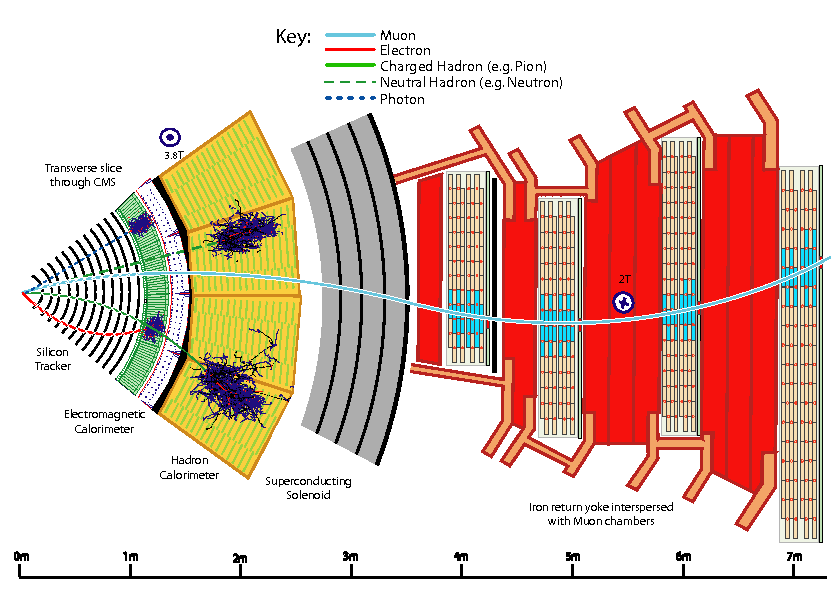
\includegraphics[width=4.0in]{cms_interaction.png}
  \caption{Representacion de la interaccion de las particulas en el detector CMS del CERN}
 \label{fig:cms_interaction}
 \end{center}
\end{figure}

\chapter{Propuesta}

En este trabajo se propone hacer un estudio por medio de simulacion de Monte Carlo de los modelos teoricos que predicen la creacion de nuevas particulas como producto de la colision de protones altamente energeticos. Estas nuevas particulas serian candidatas a explicar la composicion de la materia oscura.  Usualmente en dichos modelos las nuevas particulas interaccionan debilmente con el sector del modelo estandar, es decir con la materia visible por lo que su detecci\'on se daria de forma indirecta, o en otras palabras, por su decaimiento a particulas conocidas del modelo estandar~\cite{Curtin2015} .  Adicionalmente al estudio de los modelos teoricos se pretende trabajar en la parte experimental, la cual consiste en el estudio, de igual manera por medio de simulacion, de la respuesta del detector al paso de las particulas elementales y extraccion de los observables experimentales como los son la energia de las particulas, el momento, la trayectoria, entre otros.  La parte experimental es fundamental ya que sin una buena estrategia de selecci\'on de datos, tecnicas de supresion de ruido y optimizaci\'on de la se\~nal seria imposible la observacion de esta nueva fisica. En este proyecto se considera el detector CMS del CERN como el aparato experimental que proporcionara los datos de estudio, ya sea por simulacion o por uso de datos reales.  

En una primera fase se pretende analizar los modelos teoricos de una manera fenomenologica, es decir por medio de paquetes de simulacion propios del area de altas energias, ademas de entender la respuesta del detector a las nuevas se\~nales, buscando optimizar la seleccion de los eventos en base a las propiedades de cada modelo, en una segunda fase se pretende estudiar la se\~nal de dichos modelos bajo diferentes escenarios del detector CMS, un primer escenario seria la configuracion actual del detector CMS, que es la configuracion usada hasta el 2018, durante el llamado periodo 'Run-2'' y comparar los resultados con el detector que se tiene propuesto para la fase de alta luminosidad o tambien llamada Phase-2, la cual empezara  a partir del 2025, de esta manera se puede predecir en base a los estudios de simulacion las posibilidades de identificacion de una nueva senal en los proximos a\~nos y como la actualizacion de los detectores y metodos de identificacion de particulas podrian contribuir a incrementar las probabilidades de descubrimiento de estas nuevas particulas. 


\chapter{Justificacion}

Los estudios de nueva fisica, en particular los que predicen la produccion de nuevas particulas son bastantes relevantes dado que se aproxima la etapa de alta luminosidad del gran colisionador de hadrones, en donde se lograra acumular datos con una frecuencia 10 veces mayor en la que actualmente se esta operando, es decir la probabilidad de deteccion de nuevas se\~nales sera mucho mayor ya que se lograra alcanzar un rango de energia mayor y una cantidad de datos igualmente superior. Usualmente la probabilidad de produccion de estas particulas exoticas es baja por lo que se requiere de una cantidad grande de datos para poder observar dicha produccion. El periodo de alta luminosidad esta programado para empezar a partir del anio 2024 o 2025 como se puede ver en al linea de tiempo del Gran Acelerador de Hadrones en la Figura~\ref{fig:lhctimeline} sin embargo desde este momento se esta trabajando en la actualizacion del detector, metodos de analisis, estrategias que ayuden a optimizar la busqueda de nueva fisica. 

\begin{figure}
\begin{center}
  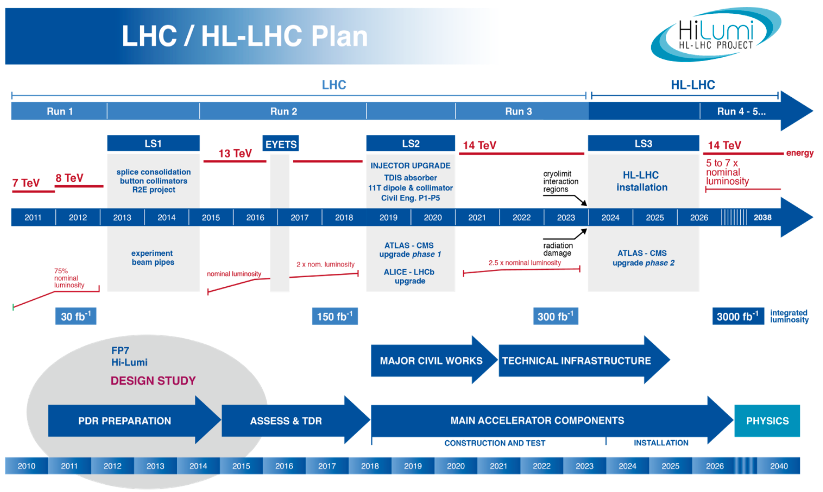
\includegraphics[width=4.0in]{lhc_timeline.png}
  \caption{Agenda de actividades del Gran Colisionador de Hadrones, donde la fase de alta luminosidad esta programada para iniciar a partir del 2024-2025}
  \label{fig:lhctimeline}
\end{center}
\end{figure}


Actualmente los modelos teoricos que predicen la formacion de particulas de materia oscura no han sido explorados ampliamente, en gran medida por falta de datos exprimentales que permitan alcanzar el espacio fase que dichos modelos predicen para esas particulas.  Actualmente con el funcionamiento del gran acelerador de hadrones y sus proyecciones en cuanto a recoleccion de datos en lo proximos anios es la perfecta oportunidad para empezar a explotar lo mas posible el estudio de dichos modelos, para en dado caso descubir una nueva senal sea facil su interpretacion en el contexto de alguno de los modelos propuesto.


\chapter{Hipotesis}

La hipotesis que se maneja en este estudio se basa en modelos solidos que postulan que la materia oscura esta compuesta de part\'{\i}culas elementales, las cuales no han sido observadas hasta este momento, sin embargo podrian ser producidas en el laboratorio, de ser esto cierto se requiere de una marco teorico, es decir una teoria mas alla del moedelo estandar que de sustento a dicha hipotesis. Afortunadamente ya existen varias modelos propuestos que predicen dicha produccion, uno de los modelos mas populares es el del llamado sector oscuro, o dark sector, por sus siglas en ingles, en el cual debido al rompimiento de una simetria se da lugar a la produccion del llamado foton oscuro (dark photon), dicha particula seria la particula portadora entre el sector oscuro y el del modelo estandar, es decir un boson, y la interaccion entre estos dos sectores se daria por medio de lo que se conoce como el parametro kinetico de mezcla (kinetic mixing paramette), usualmente abreviado como $\epsilon$~\cite{LB}, el cual mide la interaccion entre los dos sectores.

Una de las caracteristicas de esta nueva particula y que la diferencia del foton del modelo estandar es que seria masiva y que su tiempo de vida podria ser significativo, es decir la teoria tendria dos parametros libres (masa y tiempo de vida), ademas de que su deteccion se daria de forma indirecta, es decir por el decaimiento a particulas del modelo estandar.  Uno de los canales mas prometedores es en el que el foton oscuro decae a muones. los muones son particulas que pueden ser identificadas y reconstruidas con gran eficacia usando el detector CMS por lo que la probabilidad de deteccion es mayor que on otros modos de decaimientos.

\begin{figure}
\begin{center}
  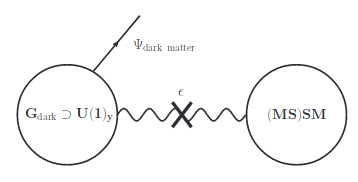
\includegraphics[width=2.8in]{sketch_darksector.png}
  \caption{Ilustracion esquematica de la conexion entre el sector oscuro y el modelo estandar, los cuales estan conectados mediente un termino de mezcla dinamica $\epsilon$}
  \label{fig:AMS_positron}
\end{center}
\end{figure}


\chapter{Objetivo General}

El objetivo general del proyecto es que se estudien, principlamente por medio de simulacion, los diferentes modelos teoricos disponibles que predicen la creacion de particulas de materia oscura en las colisiones de protones del experimento CMS del CERN.  Se buscara optimizar los parametros de los modelos y tecnicas experimentales que contribuyan a la busqueda de dicha senal en los proximos an\~nos.   Se pretende que dicho trabajo de simulacion sirva de base para un trabajo futuro mas detallado donde se incorporen tecnicas mas avanzadas de estudio. 


\chapter{Objetivos Especificos}

Se pretende alcanzar los siguiente objetivos especificos: 

\begin{itemize}
\item Entender los modelos teoricos que predicen la formacion de particulas nuevas candidatas a dar explicacion a la materia oscura, lo cual incluye ser capaz de variar los parametros e incluir dichas variaciones en paquetes de simulacion propios de la comunidad de altas energias. 
\item Desarrollar un entorno de simulacion el cual permita generar muestras estadisticas que incluyan la descripcion del modelo, generacion de eventos y simulacion del paso de particulas por el detector CMS. 
 \item Desarrollar un entorno de analisis el cual permita estudiar los eventos simulados o experimentales, el analisis incluye desde el acceso de datos, seleccion de eventos, tecnicas de supresion de ruido y tecnicas de analisis de se\~nales. 
\item Comparar los resultados con diferentes configuracion del detector CMS, se pretende comparar el detector actual con el diseno futuro en la fase de alta luminosidad, esto es posible por medio de simulaci\'on. 
  
\end{itemize}


\chapter{Metodolog\'{\i}a}

Para lograr alcanzar los objetivos deseados se pretende seguir la siguiente secuencia de actividades con el tiempo aproximado para cada una de ellas:

\begin{itemize}
  
\item Produccion de muestras de MonteCarlo (2 meses): Se espera producir muestras de simulacion de monte carlo para cada proceso de la se\~nal y ruido, el numero de eventos a producir depende del tipo de proceso que se este estudiando y su seccion eficaz, a menor seccion eficaz mayor numero de eventos que se necesitaran producir, las muestras se espera se produzcan usando los recursos computacionales de la Universidad de Sonora. Dicho paso requiere del desarrollo de codigo para la distribucion de las corridas de simulacion en forma paralela usando el cluster ACARUS. Los paquetes de simulacion que se usaran seran MADGRAPH~\cite{Alwall:2007st}, Pythia y Delphes~\cite{deFavereau2014}.

\item Analisis preliminar (2 meses): El estudiante debe desarrollar diferentes herrammientas de analisis de datos, con el fin de acceder a los datos producidos en la simulacion y extraer las variables de interes, comunmente dichas herramientas de analisis consisten de codigos escritos en lenguaje C++ y python, de esta manera el estudiante dearrollara habilidad en la manipulacion de muestras de datos 

\item Optimizacion de la seleccion de eventos (2 meses): Despues del acceso de dataos de simulacion y variables de interes se procedera al estudio de la seleccion de eventos, la cual a grandes razgos consiste en seleccionar el conjunto de variables fisicas y valores los cuales puedan optimizar el proceso de senal y reducir lo mas posible la contribucion de ruido 

\item Analisis estadistico (3 meses): Despues de la seleccion de eventos se realizara un estudio estadistico en el cual se extraeran el numero de eventos de senal y ruido despues de la seleccion, de ahi se puede interpretar los resultados en base a indicadores estadisticos y concluir la probabibilidad de obsservacion con datos recolectados en los siguientes anos terminao de

\item Escritura de Tesis (3 meses): Despues del analisis estadistico se presentara los resultados con expertos del area buscando una retroalimentacion, al mismo tiempo se procedera a la escritura del trabajo de tesis. 

\end{itemize}
  
\chapter{Resultados Esperados} 

De este proyecto se espera obtener los siguientes resultados.

\begin{itemize}
\item Identificacion de los modelos teoricos mas interesantes y cuyos parametros sean accesibles con la configuracion del detector CMS, es decir la energia de colision y los eventos proyectados a recolectar en los proximos a\~nos, de esta manera se pretende acotar los diferentes modelos disponibles.
\item Imnplementacion de un entorno de simulacion, de una manera que sea practico y reutilizable por la colaboracion para futuros estudios
\item Desarrollo de nuevas herramientas de analisis que permitan incrementar la probabiliad de deteccion de este tipode senales, es decir se buscara implementar algoritmos que contribuyan a la mejor identificacion de particulas como el foton oscuro.
\item Mejorar los paquetes de simulacion y analisis experimental ya que actualmente no se encuentran optimizados para el estudio de particulas como el foton oscuro, que debido a sus propiedades particulares (tiempo de vida largo) y se requiere de implementaciones especiales en la parte experimental.
\end{itemize}




